\documentclass[12pt, hyperref = {unicode}]{beamer}
    \pdfinterwordspaceon
    \input{glyphtounicode}
    \pdfgentounicode=1

\usepackage{geometry}

\usepackage{amsbsy}
\usepackage{amsmath}
\usepackage{amssymb}
\usepackage{amstext}
\usepackage{amsthm}
\usepackage{listings}
    \renewcommand*{\lstlistingname}{K\^{o}d}
    \renewcommand*{\lstlistlistingname}{Popis k\^{o}dova}
\usepackage{mathtools}
\usepackage[nosepfour]{numprint}
\usepackage{pgfplots}
\usepackage{pgfplotstable}
    \pgfplotsset{compat = 1.15}
\usepackage[binary-units = true, output-decimal-marker = {{,}}]{siunitx}
\usepackage{stackrel}
\usepackage{thmtools}
\usepackage{tikz}
\usepackage{units}
\usepackage{wasysym}

\usepackage{lmodern}
\usepackage[T1]{fontenc}
\usepackage[utf8]{inputenc}
\usepackage[final]{microtype}
\usepackage[croatian]{babel}

\usepackage{array}
\usepackage{chngcntr}
\usepackage{csquotes}
    \MakeOuterQuote{"}
\usepackage{graphicx}
\usepackage{subcaption}
\usepackage{marvosym}
\usepackage{multicol}
\usepackage{multirow}
\usepackage{pifont}
\usepackage{tabularx}
\usepackage{wasysym}
\usepackage{xcolor}
    \definecolor{alpha}{rgb}{0.04706, 0.13725, 0.26667}
    \definecolor{beta}{rgb}{0.506, 0.553, 0.620}
    \definecolor{gamma}{rgb}{0.380, 0.439, 0.522}
    \definecolor{delta}{rgb}{0.808, 0.827, 0.855}

\usepackage[backend = biber, indexing = true, sorting = nyvt, style = numeric, bibstyle = numeric, citestyle = numeric-comp, sortcites = true]{biblatex}

\usepackage{varioref}
\usepackage{hyperref}
    \hypersetup{
        pdfstartview = ,
        pdftitle = {Predviđanje ponašanja klijenata banke},
        pdfsubject = {Dokumentacija za predaju rješenja u sklopu kolegija Strojno učenje},
        pdfauthor = {Tim Petty},
        pdfkeywords = {Mozgalo, podatkovna znanost, rudarenje podataka, klasifikacija, binarna klasifikacija, strojno učenje, Python, CatBoost, hiperparametarska optimizacija},
        colorlinks = true,
        allcolors = beta
    }
\usepackage{cleveref}
\usepackage{url}
\usepackage{bookmark}

\usepackage{lipsum}

\mode<presentation>
\usetheme{Madrid}
\useoutertheme{infolines} % Alternatively: miniframes, infolines, split
\useinnertheme{circles}
\usefonttheme{professionalfonts}
\usecolortheme[named = alpha]{structure}

\addbibresource{literatura.bib}

\declaretheorem[style = definition, numberwithin = section, name = {Definicija}]{definicija}
\declaretheorem[style = definition, numbered = no, name = {Definicija}]{definicija*}
\declaretheorem[style = plain, sibling = definicija, name = {Teorem}]{teorem}
\declaretheorem[style = plain, numbered = no, name = {Teorem}]{teorem*}
\declaretheorem[style = plain, sibling = definicija, name = {Lema}]{lema}
\declaretheorem[style = plain, numbered = no, name = {Lema}]{lema*}
\declaretheorem[style = plain, sibling = definicija, name = {Propozicija}]{propozicija}
\declaretheorem[style = plain, numbered = no, name = {Propozicija}]{propozicija*}
\declaretheorem[style = plain, sibling = definicija, name = {Korolar}]{korolar}
\declaretheorem[style = plain, numbered = no, name = {Korolar}]{korolar*}
\declaretheorem[style = plain, sibling = definicija, name = {Slutnja}]{slutnja}
\declaretheorem[style = plain, numbered = no, name = {Slutnja}]{slutnja*}
\declaretheorem[style = remark, sibling = definicija, name = {Napomena}]{napomena}
\declaretheorem[style = remark, numbered = no, name = {Napomena}]{napomena*}
\declaretheorem[style = remark, sibling = definicija, name = {Primjer}, qed = {\ensuremath{{\lhd}}}]{primjer}
\declaretheorem[style = remark, numbered = no, name = {Primjer}, qed = {\ensuremath{{\lhd}}}]{primjer*}

\newcommand*{\naturals}{\mathbb{N}}
\newcommand*{\integers}{\mathbb{Z}}
\newcommand*{\rationals}{\mathbb{Q}}
\newcommand*{\reals}{\mathbb{R}}
\newcommand*{\complex}{\mathbb{C}}

\lstdefinestyle{lijepo}
{
    breaklines = true,
    breakatwhitespace = true,
    numbers = left,
    stepnumber = 1,
    numberstyle = {\ttfamily \bfseries \color{alpha}},
    tabsize = 4,
    frame = none,
    basicstyle = {\ttfamily \color{alpha}},
    stringstyle = {\color{gamma}},
    keywordstyle = {\bfseries \color{beta}},
    commentstyle = {\itshape \color{delta}},
    showstringspaces = true
}

\newcommand*{\fullemph}[1]{{\color{alpha} \textbf{#1}}}
\newcommand*{\halfemph}[1]{{\color{gamma} \textbf{#1}}}

\title{Predviđanje ponašanja klijenata banke}
\subtitle{Predaja rješenja u sklopu kolegija \href{http://web.math.pmf.unizg.hr/nastava/su/}{\emph{Strojno učenje}}}
\author[\emph{Petty}]{Tim \emph{Petty}}
\institute[{\hypersetup{hidelinks}\href{http://www.math.pmf.unizg.hr/}{PMF -- MO}, \href{http://www.unizg.hr/}{UniZG}}]{{\hypersetup{hidelinks}\href{http://www.math.pmf.unizg.hr/}{Prirodoslovno-matematički fakultet -- Matematički odsjek} \\ \href{http://www.unizg.hr/}{Sveučilište u Zagrebu}}}
\date{Zagreb, lipanj $ \numprint{2019} $.}

\begin{document}
    \begin{frame}
		\titlepage%
		\nocite{*}
	\end{frame}

    \section{Uvod}

    \begin{frame}{Problem -- rekapitulacija}
        Natjecanje \href{http://www.estudent.hr/category/natjecanja/mozgalo/}{\emph{Mozgalo}} $ \numprint{2019} $. godine

        \pause

        \begin{itemize}[<+->]
            \item predviđanje eventualnog prijevremenog raskida ugovora o kreditu/depozitu (\href{http://www.rba.hr/}{\emph{RBA}}) --- \fullemph{binarna klasifikacija}
            \item $ \numprint{12} $ značajki
            \begin{itemize}[<+->]
                \item $ \numprint{2} $ identifikacijske značajke
                \item $ \numprint{5} $ kategorijskih značajki
                \item $ \numprint{5} $ numeričkih odnosno vremenskih značajki
            \end{itemize}
            \item $ \numprint{5} \cdot \numprint{10}^{\numprint{6}} $ primjera za treniranje \halfemph{prije \emph{spljoštenja}}
        \end{itemize}
    \end{frame}

    \begin{frame}{Distribucije značajki}
        \only<1>{%
            \begin{figure}[htb!]
                \centering

                \begin{subfigure}{0.49\textwidth}
                    \centering
                    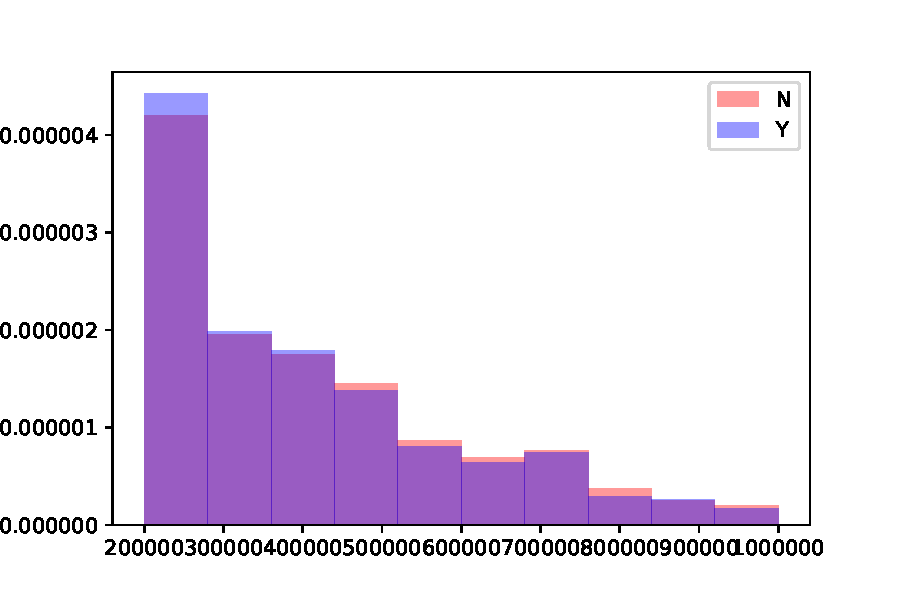
\includegraphics[width = \textwidth]{Grafovi/iznos_A.pdf}
                    \caption{\lstinline[style = lijepo, language = Python]{'A'}}
                    \label{fig:iznos_A}
                \end{subfigure}
                \hfill
                \begin{subfigure}{0.49\textwidth}
                    \centering
                    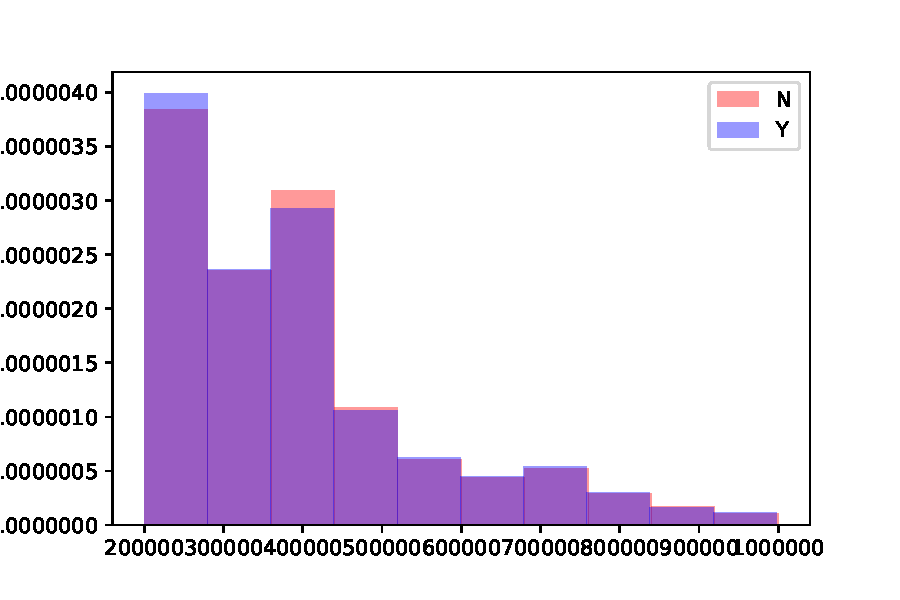
\includegraphics[width = \textwidth]{Grafovi/iznos_L.pdf}
                    \caption{\lstinline[style = lijepo, language = Python]{'L'}}
                    \label{fig:iznos_L}
                \end{subfigure}

                \par

                \caption{Ugovoreni iznos}
                \label{fig:iznos}
            \end{figure}
        }%
        \only<2>{%
            \begin{figure}[htb!]
                \centering

                \begin{subfigure}{0.49\textwidth}
                    \centering
                    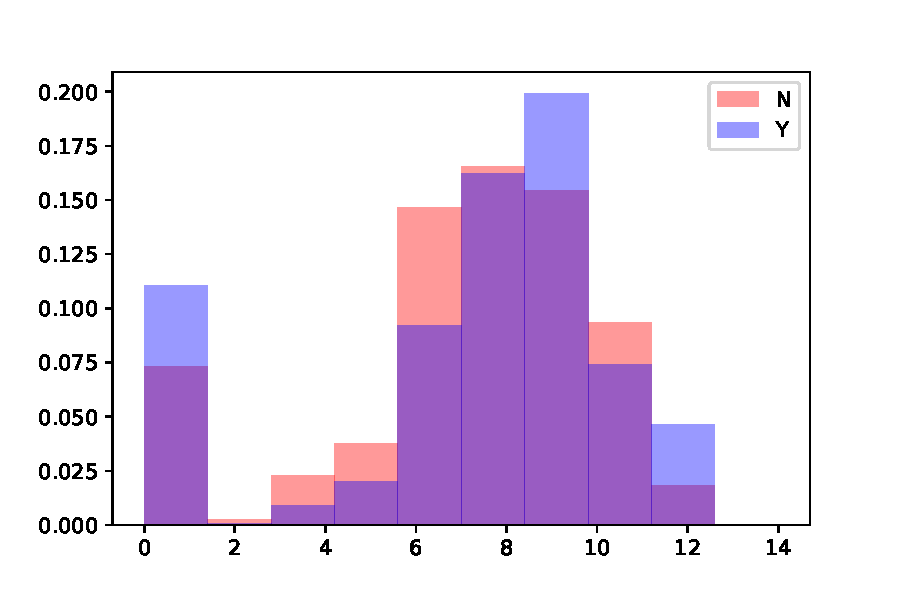
\includegraphics[width = \textwidth]{Grafovi/kamata_A.pdf}
                    \caption{\lstinline[style = lijepo, language = Python]{'A'}}
                    \label{fig:kamata_A}
                \end{subfigure}
                \hfill
                \begin{subfigure}{0.49\textwidth}
                    \centering
                    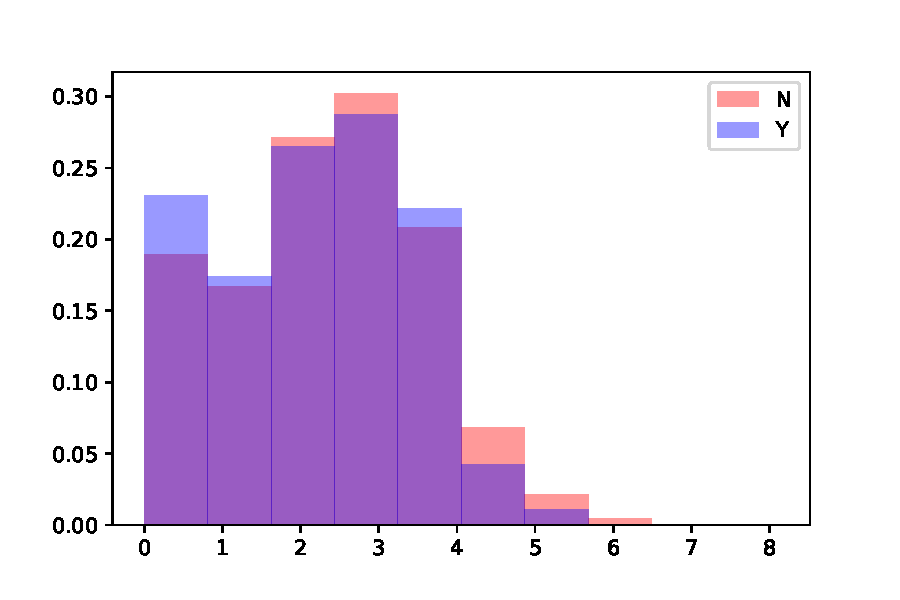
\includegraphics[width = \textwidth]{Grafovi/kamata_L.pdf}
                    \caption{\lstinline[style = lijepo, language = Python]{'L'}}
                    \label{fig:kamata_L}
                \end{subfigure}

                \par

                \caption{Visina kamate}
                \label{fig:kamata}
            \end{figure}
        }%
        \only<3>{%
            \begin{figure}[htb!]
                \centering

                \begin{subfigure}{0.49\textwidth}
                    \centering
                    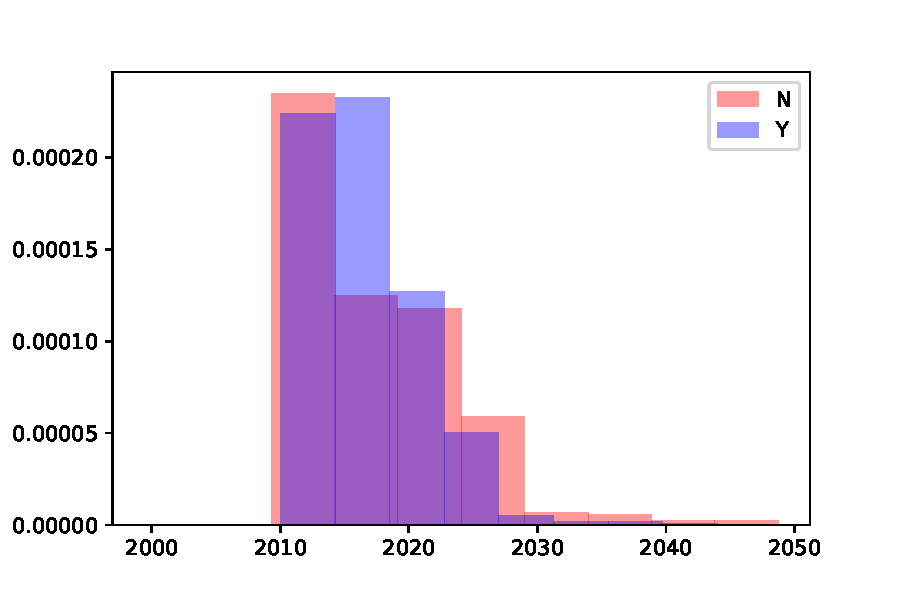
\includegraphics[width = \textwidth]{Grafovi/planirani_datum_zatvaranja_A.pdf}
                    \caption{\lstinline[style = lijepo, language = Python]{'A'}}
                    \label{fig:planirani_datum_zatvaranja_A}
                \end{subfigure}
                \hfill
                \begin{subfigure}{0.49\textwidth}
                    \centering
                    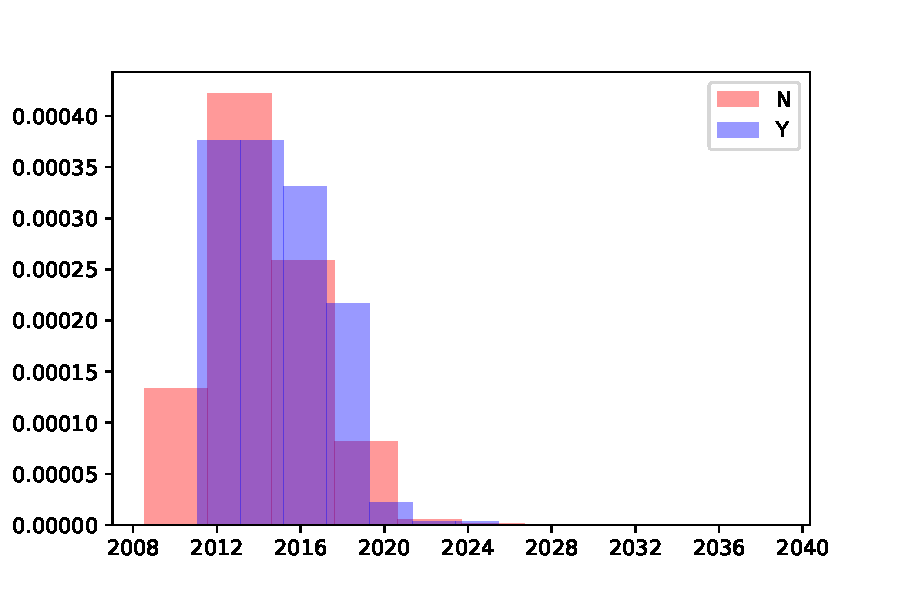
\includegraphics[width = \textwidth]{Grafovi/planirani_datum_zatvaranja_L.pdf}
                    \caption{\lstinline[style = lijepo, language = Python]{'L'}}
                    \label{fig:planirani_datum_zatvaranja_L}
                \end{subfigure}

                \par

                \caption{Planirani datum zatvaranja}
                \label{fig:planirani_datum_zatvaranja}
            \end{figure}
        }
    \end{frame}

    \section{Razvoj modela}

    \begin{frame}{Značajčko inženjerstvo}
        \begin{enumerate}[<+->]
            \item \fullemph{spljoštenje}
            \begin{itemize}[<+->]
                \item svi primjeri s istom oznakom partije spljošte se u $ \numprint{1} $ primjer
                \item pamte se prva i zadnja varirajuća značajka
            \end{itemize}
            \item makroekonomske značajke
            \begin{itemize}[<+->]
                \item BDP
                \item inflacija
                \item nezaposlenost
                \item cijena nafte
            \end{itemize}
            \item kombinacije značajki
            \begin{itemize}[<+->]
                \item trajanje, trajanje u krizi, promjene značajki
                \item kamatni račun
                \item matematički račun nad značajkama baziran na statistici i intuiciji
            \end{itemize}
        \end{enumerate}
    \end{frame}

    \begin{frame}{{\hypersetup{hidelinks}\href{http://catboost.ai/}{\emph{CatBoost}}}}
        \begin{itemize}[<+->]
            \item \href{http://catboost.ai/docs/concepts/python-reference_catboostclassifier.html}{\lstinline[style = lijepo, language = Python]{CatBoostClassifier}} --- ansambl stabala odlučivanja razvijen \emph{jačanjem} (eng.\ \emph{boosting})
            \item $ \numprint{3} $ modela
            \begin{itemize}[<+->]
                \item za kredite do $ \numprint{6} $.\ listopada $ \numprint{2016} $.
                \item za depozite do $ \numprint{6} $.\ listopada $ \numprint{2016} $.
                \item za ostale ugovore
            \end{itemize}
            \item svi su modeli konstruirani simetričnim stablima --- \halfemph{interpretabilnost}
        \end{itemize}
    \end{frame}

    \begin{frame}{Hiperparametri}
        \only<1>{%
            \lstinputlisting[style = lijepo, stepnumber = 0, basicstyle = {\footnotesize \ttfamily \color{alpha}}, language = Python, caption = {Primjer konstrukcije modela}, label = {lst:model}]{Kodovi/model.py}%
        }%
        \only<2>{%
            \lstinputlisting[style = lijepo, stepnumber = 0, basicstyle = {\footnotesize \ttfamily \color{alpha}}, language = Python, caption = {Primjer treniranja modela}, label = {lst:fit}]{Kodovi/fit.py}%
        }
    \end{frame}

    %http://towardsdatascience.com/a-conceptual-explanation-of-bayesian-model-based-hyperparameter-optimization-for-machine-learning-b8172278050f
    \begin{frame}{Optimizacija hiperparametara}
        \textbf{\href{http://hyperopt.github.io/hyperopt/}{\fullemph{\emph{Hyperopt}}}}
        \pause
        \begin{itemize}[<+->]
            \item \href{http://www.python.org/}{\emph{Python}} biblioteka za optimizaciju
            \item pogodna za kompleksne prostore pretraživanja
            \item realne, diskretne i uvjetne domene
            \item \emph{Bayesovska} optimizacija
        \end{itemize}
    \end{frame}

    \section{Rezultati}
    \begin{frame}{Rezultati}{Konfuzijske tablice}
        \only<1>{%
            \begin{table}[htb!]
                \centering
                \caption{Model A}
                \label{tab:konfuzijska_tablica_A}
                \begin{tabular}{r | c | c c | c |}
                    \multicolumn{2}{l}{} & \multicolumn{2}{c}{Stvarno} & \multicolumn{1}{l}{} \\
                    \cline{3-4}
                    \multicolumn{2}{l |}{} & $ \boldsymbol{N} $ & $ \boldsymbol{Y} $ & \multicolumn{1}{l}{} \\
                    \cline{2-5}
                    \multirow{2}{*}{Predikcija} & $ \boldsymbol{N} $ & $ \mathbf{\numprint{7408}} $ & $ \numprint{2349} $ & $ \numprint{9757} $ \\
                    & $ \boldsymbol{Y} $ & $ \numprint{2833} $ & $ \mathbf{\numprint{12143}} $ & $ \numprint{14976} $ \\
                    \cline{2-5}
                    \multicolumn{2}{l |}{} & $ \numprint{10241} $ & $ \numprint{14492} $ & $ \mathbf{\numprint{24733}} $ \\
                    \cline{3-5}
                \end{tabular}
            \end{table}
        }%
        \only<2>{%
            \begin{table}[htb!]
                \centering
                \caption{Model L}
                \label{tab:konfuzijska_tablica_L}
                \begin{tabular}{r | c | c c | c |}
                    \multicolumn{2}{l}{} & \multicolumn{2}{c}{Stvarno} & \multicolumn{1}{l}{} \\
                    \cline{3-4}
                    \multicolumn{2}{l |}{} & $ \boldsymbol{N} $ & $ \boldsymbol{Y} $ & \multicolumn{1}{l}{} \\
                    \cline{2-5}
                    \multirow{2}{*}{Predikcija} & $ \boldsymbol{N} $ & $ \mathbf{\numprint{8066}} $ & $ \numprint{1510} $ & $ \numprint{9576} $ \\
                    & $ \boldsymbol{Y} $ & $ \numprint{2430} $ & $ \mathbf{\numprint{14800}} $ & $ \numprint{17230} $ \\
                    \cline{2-5}
                    \multicolumn{2}{l |}{} & $ \numprint{10496} $ & $ \numprint{16310} $ & $ \mathbf{\numprint{26806}} $ \\
                    \cline{3-5}
                \end{tabular}
            \end{table}
        }%
        \only<3>{%
            \begin{table}[htb!]
                \centering
                \caption{Ostali}
                \label{tab:konfuzijska_tablica_ostali}
                \begin{tabular}{r | c | c c | c |}
                    \multicolumn{2}{l}{} & \multicolumn{2}{c}{Stvarno} & \multicolumn{1}{l}{} \\
                    \cline{3-4}
                    \multicolumn{2}{l |}{} & $ \boldsymbol{N} $ & $ \boldsymbol{Y} $ & \multicolumn{1}{l}{} \\
                    \cline{2-5}
                    \multirow{2}{*}{Predikcija} & $ \boldsymbol{N} $ & $ \mathbf{\numprint{10748}} $ & $ \numprint{3700} $ & $ \numprint{14448} $ \\
                    & $ \boldsymbol{Y} $ & $ \numprint{2598} $ & $ \mathbf{\numprint{7154}} $ & $ \numprint{9752} $ \\
                    \cline{2-5}
                    \multicolumn{2}{l |}{} & $ \numprint{13346} $ & $ \numprint{10854} $ & $ \mathbf{\numprint{24200}} $ \\
                    \cline{3-5}
                \end{tabular}
            \end{table}
        }%
        \only<4>{%
            \begin{table}[htb!]
                \centering
                \caption{Ukupno}
                \label{tab:konfuzijska_tablica_ukupno}
                \begin{tabular}{r | c | c c | c |}
                    \multicolumn{2}{l}{} & \multicolumn{2}{c}{Stvarno} & \multicolumn{1}{l}{} \\
                    \cline{3-4}
                    \multicolumn{2}{l |}{} & $ \boldsymbol{N} $ & $ \boldsymbol{Y} $ & \multicolumn{1}{l}{} \\
                    \cline{2-5}
                    \multirow{2}{*}{Predikcija} & $ \boldsymbol{N} $ & $ \mathbf{\numprint{26222}} $ & $ \numprint{7559} $ & $ \numprint{33781} $ \\
                    & $ \boldsymbol{Y} $ & $ \numprint{7861} $ & $ \mathbf{\numprint{34097}} $ & $ \numprint{41958} $ \\
                    \cline{2-5}
                    \multicolumn{2}{l |}{} & $ \numprint{34083} $ & $ \numprint{41656} $ & $ \mathbf{\numprint{75739}} $ \\
                    \cline{3-5}
                \end{tabular}
            \end{table}
        }
    \end{frame}
        
    \begin{frame}{Rezultati}{Vlastiti validacijski \emph{dataset}}
        \begin{table}[htb!]
            \centering
            \caption{Evaluacijske mjere modela}
            \label{tab:rezultati_vlastita_validacija}
            \begin{tabular}{| l | c | c | c | c |}
                \hline
                \textbf{Model} & Točnost & Preciznost & Odziv & $ F_{\numprint{1}} $ \\
                \hline
                \textbf{A} & $ \unit[\numprint{85.3}]{\%} $ & $ \unit[\numprint{85.9}]{\%} $ & $ \unit[\numprint{90.7}]{\%} $ & $ \unit[\numprint{88.3}]{\%} $ \\
                \textbf{L} & $ \unit[\numprint{74.0}]{\%} $ & $ \unit[\numprint{73.4}]{\%} $ & $ \unit[\numprint{66.0}]{\%} $ & $ \unit[\numprint{69.4}]{\%} $ \\
                \textbf{Ostali} & $ \unit[\numprint{79.0}]{\%} $ & $ \unit[\numprint{81.1}]{\%} $ & $ \unit[\numprint{83.8}]{\%} $ & $ \unit[\numprint{82.4}]{\%} $ \\
                \hline
                \textbf{Ukupno} & $ \unit[\numprint{79.6}]{\%} $ & $ \unit[\numprint{81.3}]{\%} $ & $ \unit[\numprint{81.9}]{\%} $ & $ \unit[\numprint{81.6}]{\%} $ \\
                \hline
            \end{tabular}
        \end{table}
    \end{frame}

    \begin{frame}{Rezultati}{{\hypersetup{hidelinks}\href{http://www.estudent.hr/category/natjecanja/mozgalo/}{\emph{Mozgalo}} $ \numprint{2019} $.\ -- evaluacijski i validacijski \emph{dataset}}}
        \begin{table}[htb!]
            \centering
            \caption{Rezultati na natjecanju}
            \label{tab:rezultati_evaluacija_i_validacija}
            \begin{tabular}{| l | c | c | c |}
                \hline
                \multicolumn{1}{| c |}{\ding{70}} & Točnost & $ F_{\numprint{1}} $ & Ostvareni bodovi \\
                \hline
                Evaluacija & $ \unit[\numprint{71}]{\%} $ & $ \unit[\numprint{77}]{\%} $ & $ \numprint{14} / \numprint{15} $ \\
                Validacija & $ \unit[\numprint{69}]{\%} $ & $ \unit[\numprint{70}]{\%} $ & $ \numprint{17} / \numprint{20} $ \\
                \hline
                \multicolumn{3}{l |}{ } & $ \mathbf{\numprint{31}} / \mathbf{\numprint{35}} $ \\
                \cline{4-4}
            \end{tabular}
        \end{table}
    \end{frame}

    \begin{frame}{Ukupni plasman}
        Nismo ušli u finale --- bili smo $ \numprint{8} $., a $ \numprint{6} $ je finalista

        \pause
        \bigskip

        \begin{center}
            \Huge
            \frownie
        \end{center}
    \end{frame}

    \begin{frame}{Komentari i pitanja}
        \centering
        \begin{tikzpicture}[scale = 0.05]
        \draw (48.656200, 67.906197)..controls (48.656200, 75.199203) and (43.636700, 84.164101)..(26.421900, 84.164101)
            ..controls (13.507800, 84.164101) and (6.457030, 75.796898)..(6.457030, 68.144501)
            ..controls (6.457030, 63.839802) and (9.683590, 62.882801)..(11.476600, 62.882801)
            ..controls (13.507800, 62.882801) and (16.378901, 64.320297)..(16.378901, 67.906197)
            ..controls (16.378901, 70.656197) and (14.347700, 72.808601)..(11.359400, 72.808601)
            ..controls (10.640600, 72.808601) and (10.402300, 72.808601)..(10.160200, 72.687500)
            ..controls (12.793000, 78.902298) and (19.726601, 81.773399)..(26.062500, 81.773399)
            ..controls (39.570301, 81.773399) and (39.570301, 73.046898)..(39.570301, 68.503899)
            ..controls (39.570301, 61.449200) and (37.417999, 59.179699)..(35.386700, 57.027302)
            ..controls (27.257799, 48.300800) and (24.628901, 37.179699)..(24.628901, 29.886700)
            --(24.628901, 24.148399)..controls (24.628901, 21.996099) and (24.628901, 21.519501)..(25.941401, 21.519501)
            ..controls (27.257799, 21.519501) and (27.257799, 22.355499)..(27.257799, 24.507799)
            --(27.257799, 28.929701)..controls (27.257799, 35.984402) and (30.128901, 46.503899)..(42.203098, 55.472698)
            ..controls (45.550800, 57.984402) and (48.656200, 61.687500)..(48.656200, 67.906197)
            --cycle;
        \draw (31.679701, 5.859380)..controls (31.679701, 8.964840) and (29.050800, 11.597700)..(25.941401, 11.597700)
            ..controls (22.355499, 11.597700) and (20.085899, 8.726560)..(20.085899, 5.859380)
            ..controls (20.085899, 2.269530) and (22.953100, 0.000000)..(25.824200, 0.000000)
            ..controls (29.171900, 0.000000) and (31.679701, 2.628910)..(31.679701, 5.859380)
            --cycle;
        \end{tikzpicture}
    \end{frame}

    \section{Implementacija}

    \begin{frame}{Programska realizacija}
        \centering
        \Huge
        \href{run:jupyter.sh}{Implementacija \ding{40}}
    \end{frame}{}

    \begin{frame}[allowframebreaks]{Literatura}
        \printbibliography
    \end{frame}
\end{document}
